\chapter{Przegląd literatury}
Celem niniejszego rozdziału jest przedstawienie dotychczasowych badań i publikacji dotyczących mechanizmów programowania współbieżnego i równoległego w językach Rust i C++. Analiza literatury umożliwi zrozumienie aktualnego stanu wiedzy w tej dziedzinie, a także wskazanie na występujące luki badawcze, które niniejsza praca postara się wypełnić.

Przegląd literatury odbywał się z wykorzystaniem narzędzi baz danych oferujących wyszukiwanie, filtrowanie oraz przegląd prac: Scopus, Google Scholar.\\
W ramach bazy scopus wykorzystano następujące kwerendy do wyszukiwania - tabela \ref{table:literatureReviewQueries}

\begin{table}[H]
    \caption{Kwerendy użyte w bazie Scopus \protect \footnotemark}
    \label{table:literatureReviewQueries}
    \begin{tabular}{|c|p{11cm}|c|}
    \hline
    Lp. & Kwerenda & Liczba wyników \\ \hline
    1 & ALL ("concurrent programming"\ OR "parallel programming") AND (ALL ("Rust") AND ALL ("C++")) & 444 \\ \hline
    2 & ALL ("concurrent programming"\ OR "parallel programming") AND (ALL ("Rust") AND ALL ("C++") ) AND ( ALL ("compare")) & 28 \\ \hline
    \end{tabular}
\end{table}
\footnotetext{Ilość wyników dla poszczególnych zapytań może się różnić w zależności od daty (wyszukiwanie przeprowadzono w okresie listopad-luty 2024/25).}

Autor zdecydował się również użyć nowego, wbudowane narzędzia w systemie Scopus - Scopus AI. Narzędzie to oparte na sztucznej inteligencji, wspomaga eksplorację akademicką w oparciu o dane z platformy Scopus. Dzięki integracji z narzędziem Copilot optymalizuje wyszukiwania, łącząc metody semantyczne i dopasowanie słów kluczowych. Choć Scopus AI ułatwia badania, jego wyniki warto weryfikować, ponieważ mogą zawierać nieścisłości lub stronniczość. \\
Po wprowadzeniu tytułu pracy w języku angielskim jako kwerendę, Scopus AI zwrócił 9 wyników, biorąc pod uwagę kwerendę stworzoną na podstawie tytyułu pracy, zamieszczoną w listingu \ref{AIQuery}. Zwrócone prace pokrywają się z przeglądem umieszczonym w tabeli \ref{table:literatureReviewQueries} 

\lstset{breaklines=true}
\begin{lstlisting}[caption=Kwerenda wygenerowana przez AI, label=AIQuery]
("concurrent programming" OR "parallel programming" OR "multithreading" OR "asynchronous")
AND ("Rust" OR "C++" OR "programming languages" OR "software development")
AND ("performance" OR "efficiency" OR "scalability" OR "resource management")
AND ("synchronization" OR "thread safety" OR "deadlock" OR "race condition")
AND ("libraries" OR "frameworks" OR "tools" OR "APIs")
\end{lstlisting}


\section{Porównanie Rust oraz C++}
Porównanie języków programowania Rust i C++ jest przedmiotem licznych publikacji, które analizują ich różnorodne aspekty, takie jak struktura kodu, sposób kompilacji, bezpieczeństwo, wydajność oraz obsługa współbieżności i równoległości.

Jednym z podstawowych kryteriów porównań jest model kompilacji. Rust i C++ są językami kompilowanymi, co oznacza, że dedykowany kompilator tłumaczy kod źródłowy na kod maszynowy przed jego wykonaniem. Dzięki temu możliwe jest uzyskanie wysokiej wydajności programów. W literaturze \cite{Lesiński} często podkreśla się, że Rust, w odróżnieniu od C++, kładzie większy nacisk na bezpieczeństwo pamięci oraz typów w czasie kompilacji, co ma kluczowe znaczenie w nowoczesnym oprogramowaniu. W kontekście C++ wskazuje się na jego większą elastyczność oraz bogaty ekosystem, który pozwala na szeroką gamę zastosowań, ale jednocześnie wymaga większej uwagi programistów w zakresie zarządzania pamięcią i synchronizacji wątków.
% two images next to each other
\begin{figure}[H]
    \centering
    \begin{minipage}{.5\textwidth}
        \centering
        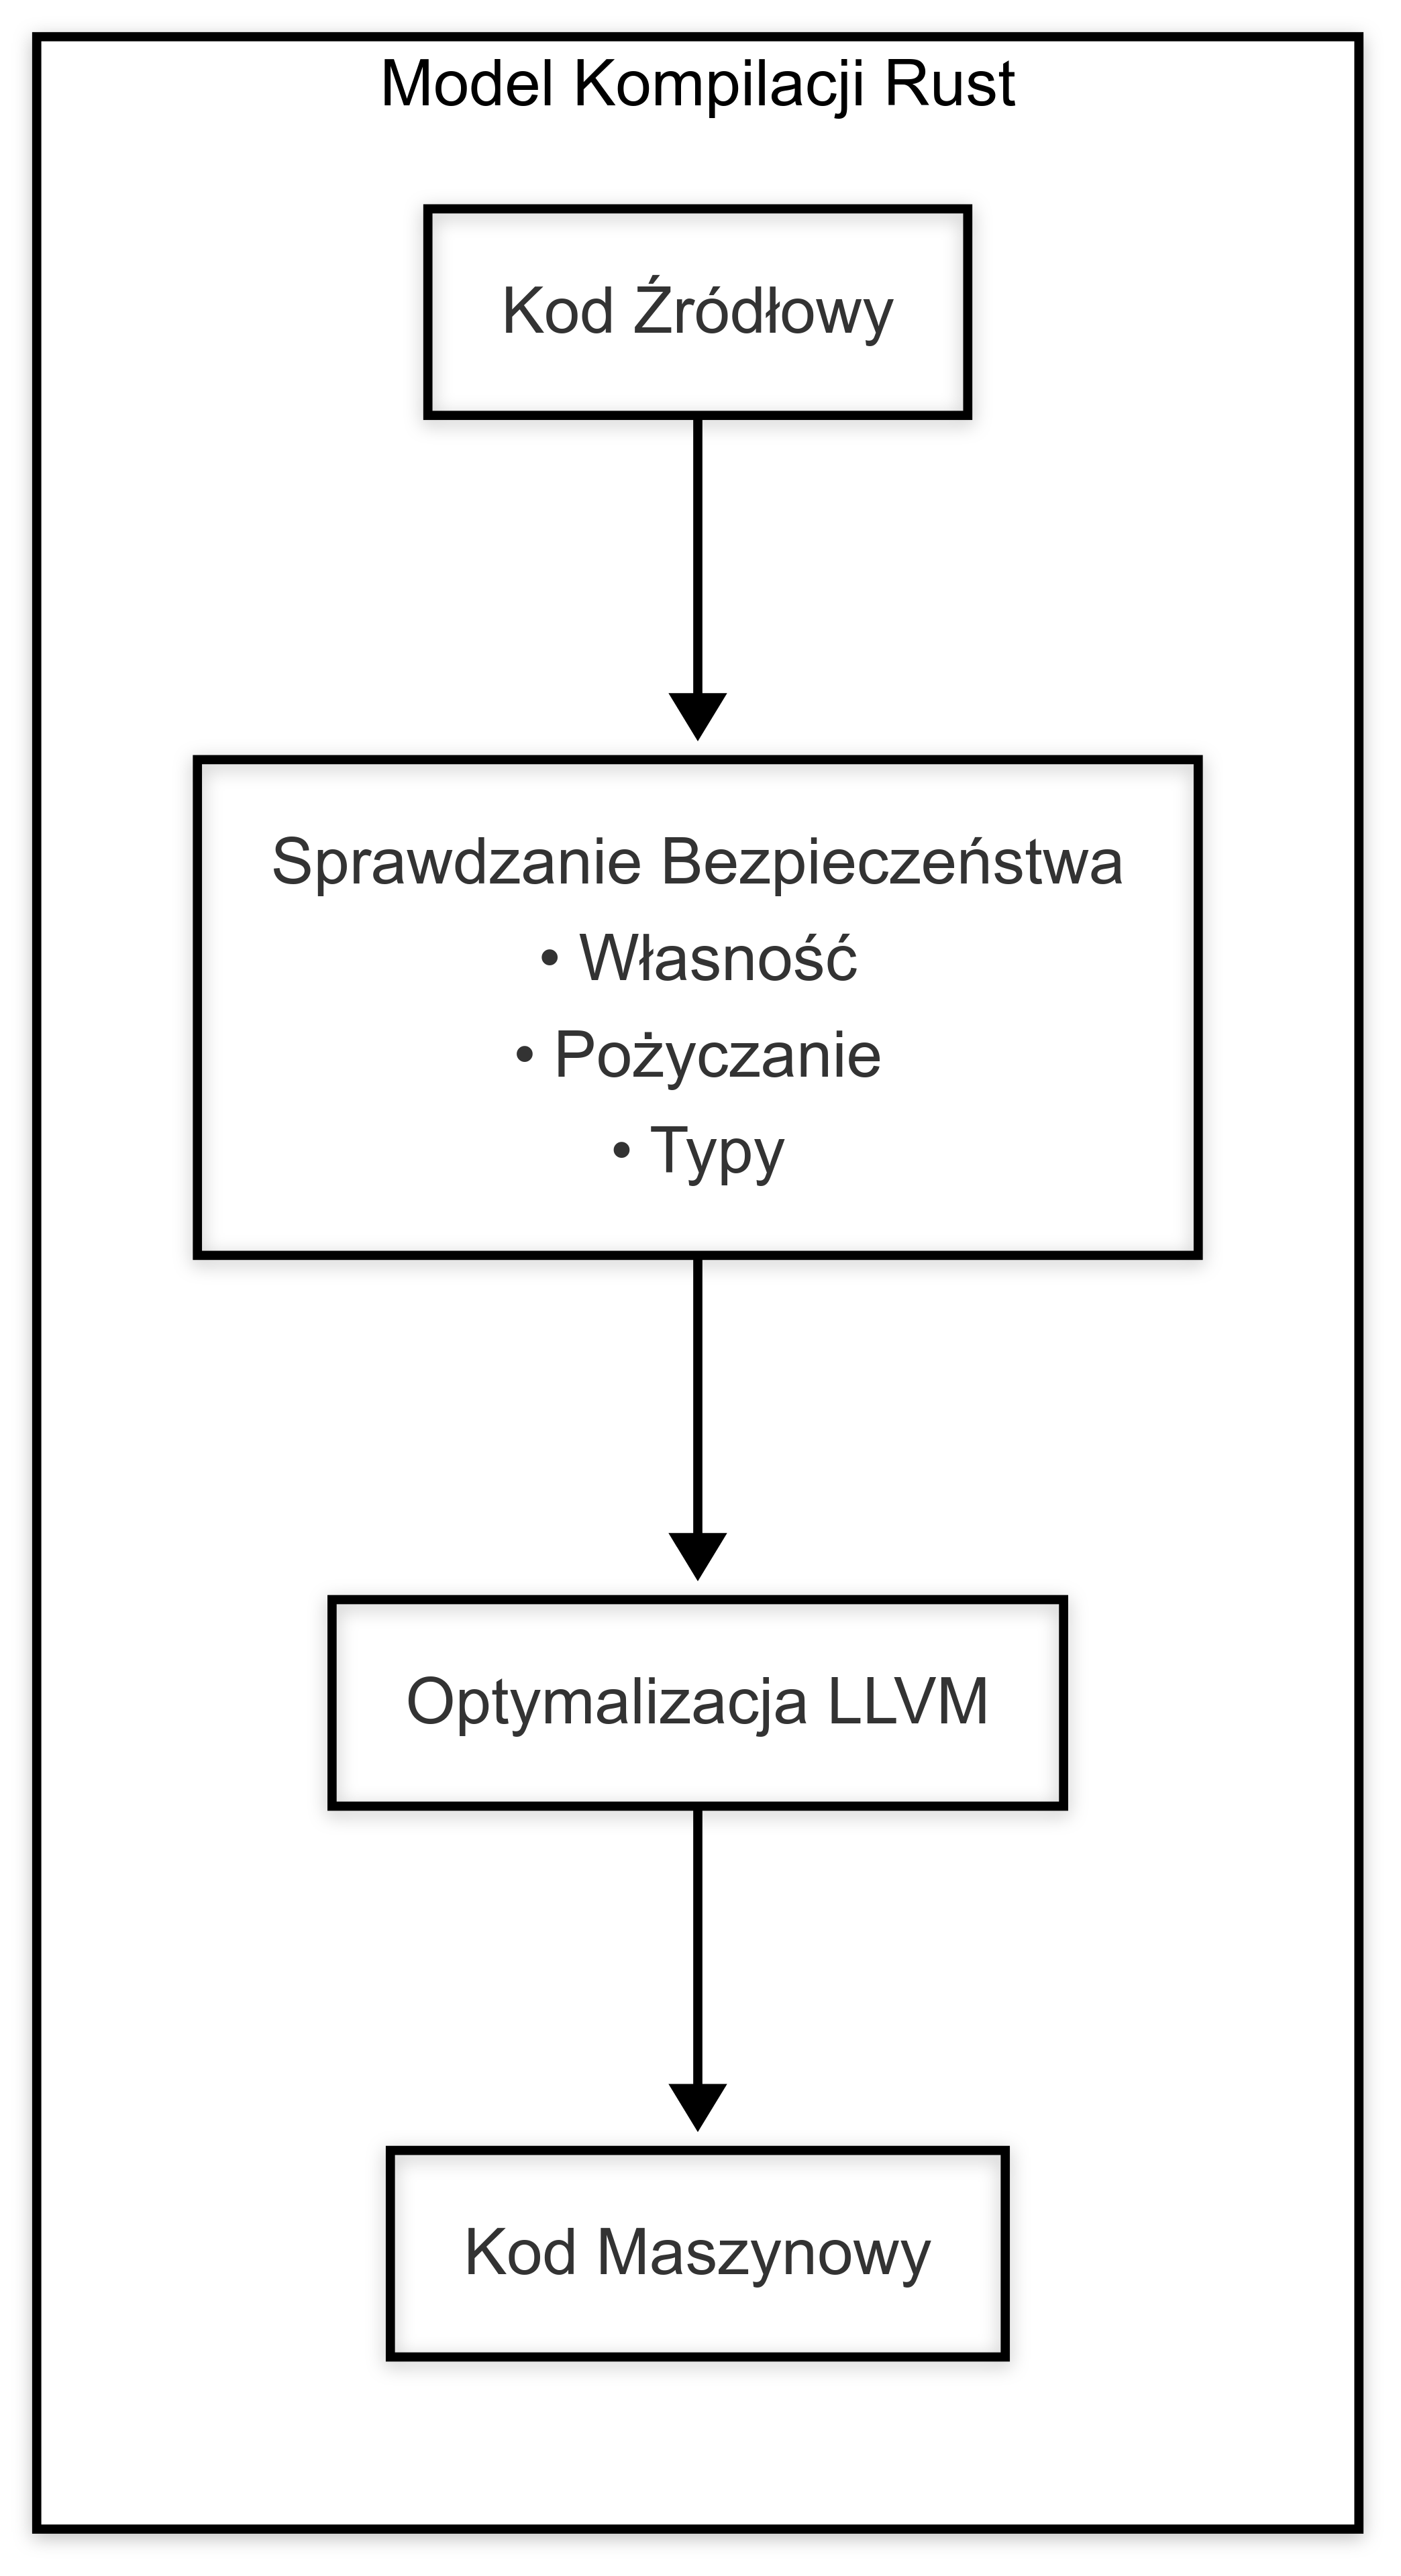
\includegraphics[height=12cm]{images/RustBuildsSteps.png}
        \caption{Kroki kompilacji w języku Rust}
        \label{fig:rust_build_steps}
    \end{minipage}%
    \begin{minipage}{.5\textwidth}
        \centering
        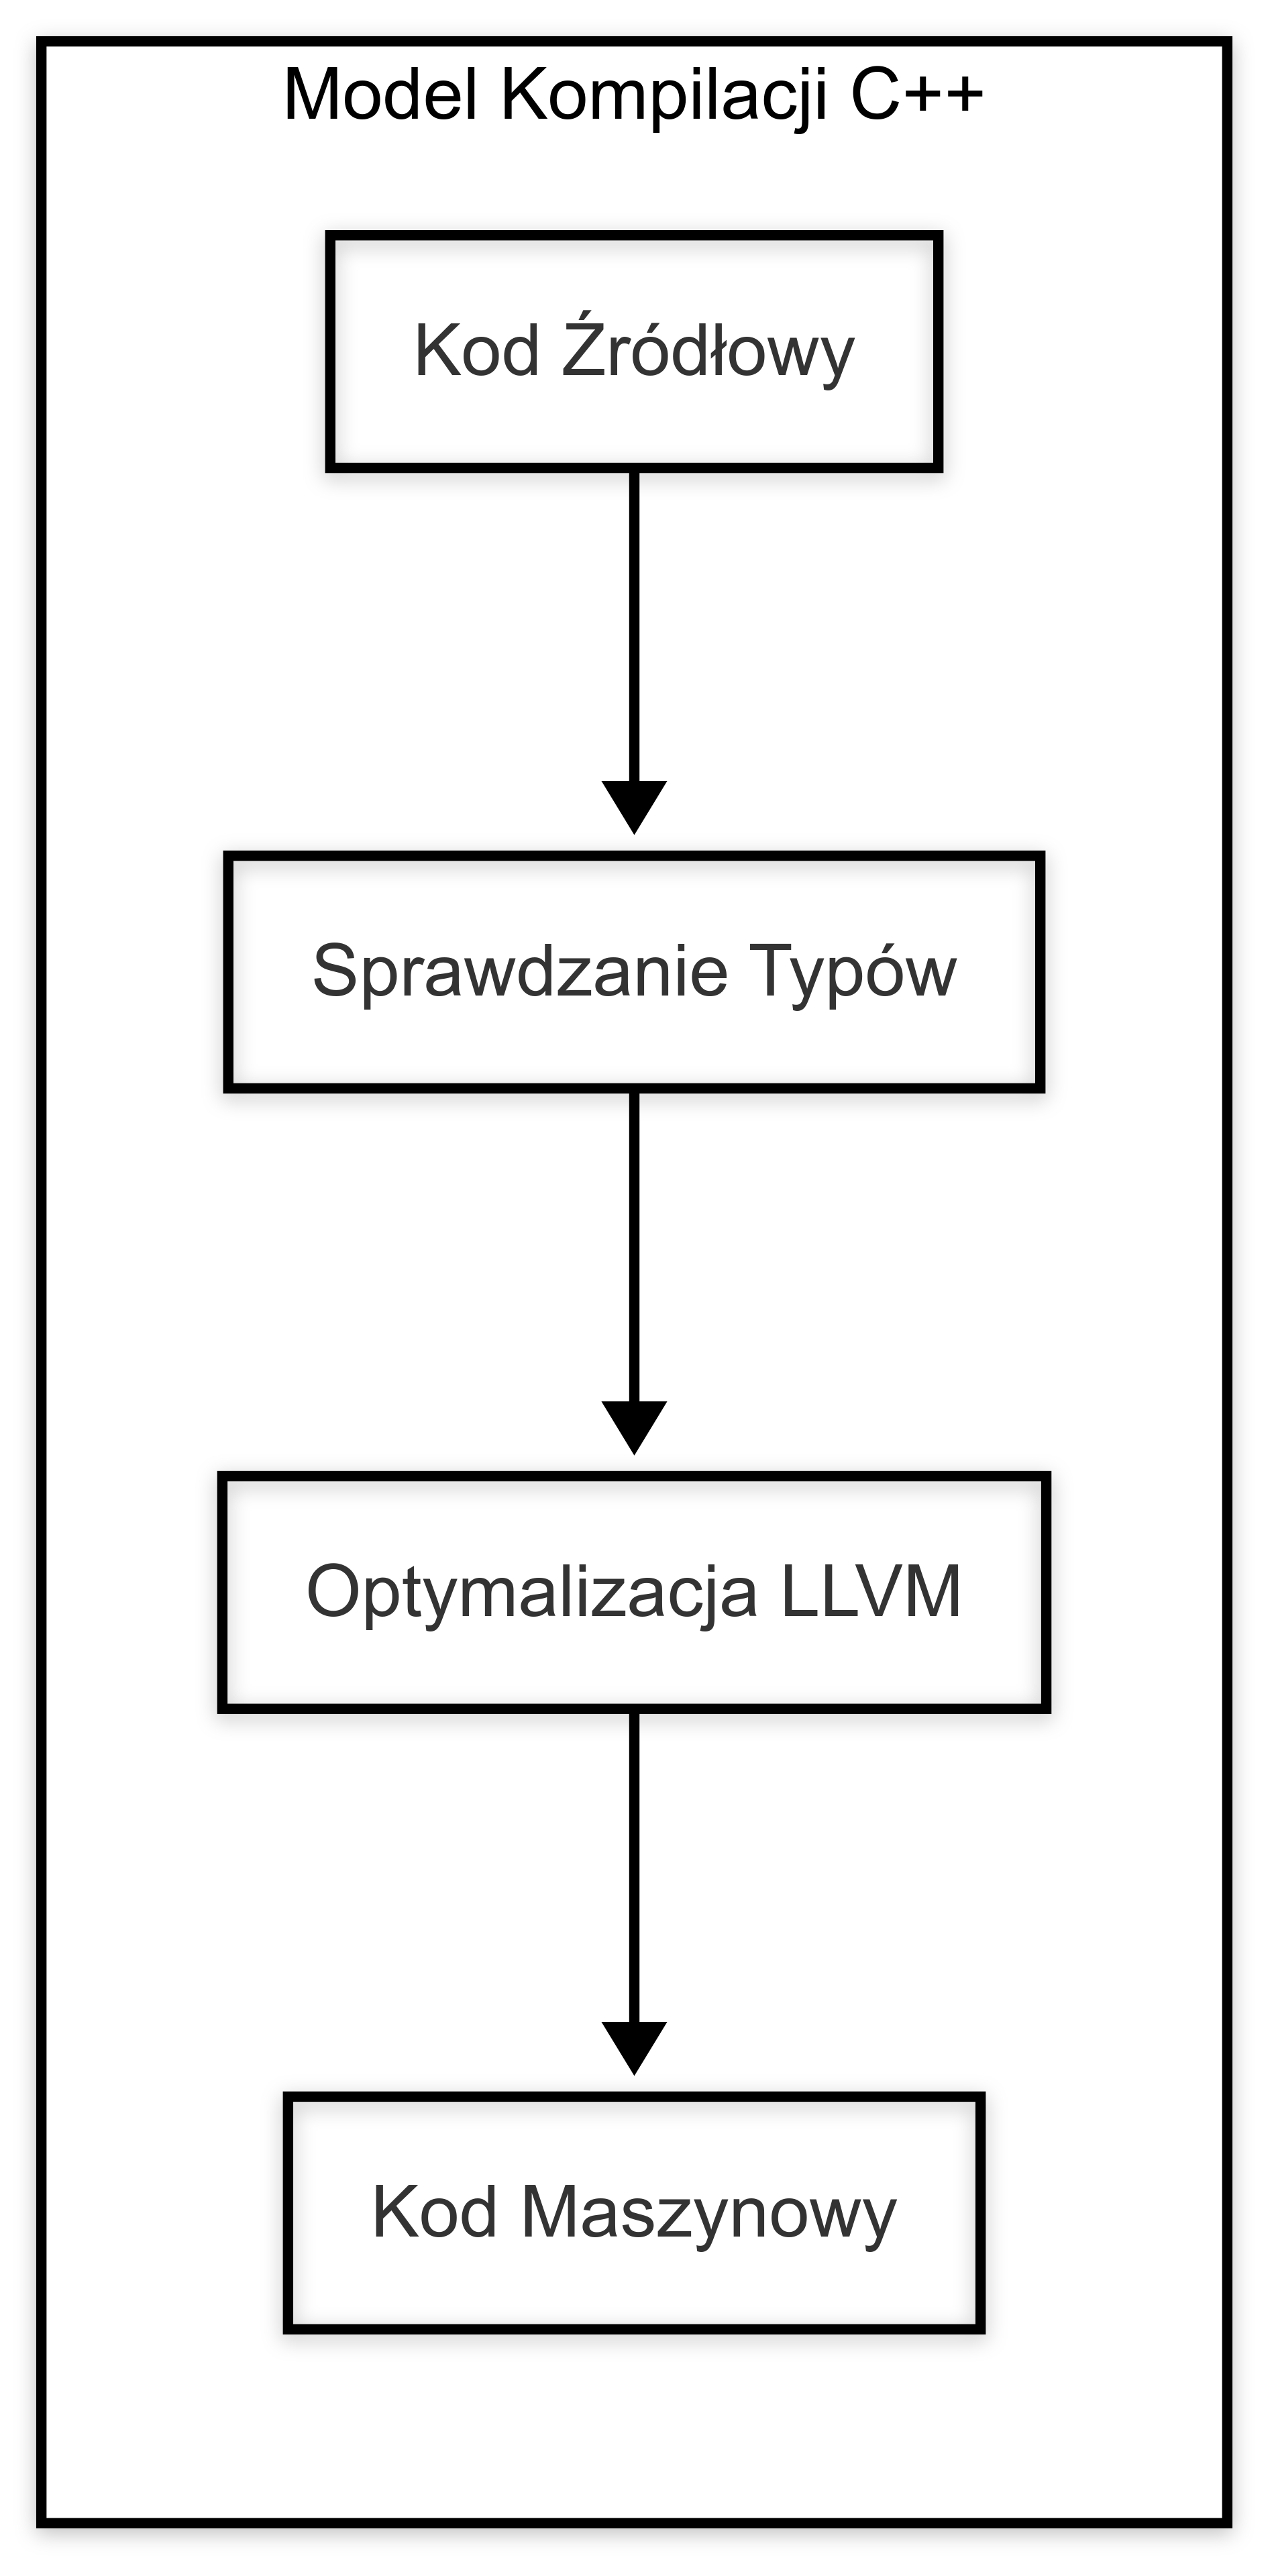
\includegraphics[height=12cm]{images/CppBuildsSteps.png}
        \caption{Kroki kompilacji w języku C++}
        \label{fig:cpp_build_steps}
    \end{minipage}
    \caption{Porównanie kroków kompilacji w językach Rust i C++}
\end{figure}

Informacje o procesie kompilacji pochodzą z \cite{Lesiński, rustPolishNames, TheRustProgrammingLanguage}, które opisują integrację z LLVM i różnice w sprawdzaniu bezpieczeństwa.
Na diagramie \ref{fig:rust_build_steps} drugi blok reprezentuje dodatkowe etapy sprawdzania bezpieczeństwa w Rust, które nie występują w C++. Z kolei na diagramie \ref{fig:cpp_build_steps} drugi blok pokazuje podstawowe sprawdzanie typów w C++, które jest mniej rygorystyczne niż system Rust.

Kolejnym ważnym aspektem poruszanym w badaniach są różnice w modelach obsługi błędów. Rust implementuje mechanizm ownership oraz lifetimes, które pozwalają na jednoznaczne zarządzanie cyklem życia zasobów w czasie kompilacji, minimalizując ryzyko wycieków pamięci \cite{MigratingCtoRustforMemorySafety}. C++ oferuje alternatywne rozwiązania, takie jak wskaźniki inteligentne (smart pointers), ale pozostawia programiście większą swobodę, co może prowadzić do potencjalnych błędów. \cite{RustDifferences, RustDifferences1}

\subsection{Bezpieczeństwo}
Bezpieczeństwo języków Rust i C++ jest jednym z najczęściej analizowanych tematów w literaturze. W przypadku Rusta duży nacisk kładziony jest na eliminację całych klas błędów, takich jak null pointer dereferencing, data races oraz wycieki pamięci. Mechanizmy takie jak ownership, borrow checker oraz obowiązkowa mutowalność zmiennych (explicit mutability) są wymieniane jako kluczowe elementy zapewniające bezpieczeństwo.

Z drugiej strony, C++ umożliwia większą kontrolę nad pamięcią, co może być zaletą w systemach wymagających maksymalnej wydajności, ale jednocześnie wiąże się z koniecznością samodzielnego zarządzania zasobami przez programistów. W literaturze często podkreśla się, że to właśnie większa złożoność i ryzyko błędów w kodzie C++ skłoniły społeczność do stworzenia języków takich jak Rust.

Przykładowo, badania wskazują, że aplikacje napisane w Rusta są mniej podatne na błędy związane z wyścigami danych (data races), co ma szczególne znaczenie w środowiskach wielowątkowych. Z kolei w C++ stosowanie bibliotek takich jak std::thread czy frameworków typu OpenMP pozwala na osiągnięcie podobnych celów, choć wymaga od programistów większej uwagi w zakresie synchronizacji. \cite{RustSafety1, RustSafety2, RustSafety3}

\subsection{Czas wykonania}
Porównania czasów wykonania programów napisanych w Rust i C++ są częstym tematem analiz. W większości badań wskazuje się, że pod względem wydajności Rust jest konkurencyjny wobec C++, co wynika z podobnych mechanizmów kompilacji i optymalizacji kodu.

Jednak kluczową różnicą jest to, że Rust wprowadza pewne narzuty związane z kontrolą bezpieczeństwa w czasie kompilacji, które mogą wydłużyć czas budowania programu, ale nie wpływają znacząco na czas wykonania. W badaniach eksperymentalnych często porównuje się wydajność aplikacji w obliczeniach numerycznych, przetwarzaniu danych oraz w zadaniach wymagających intensywnego dostępu do pamięci.

C++ nadal pozostaje językiem preferowanym w projektach o krytycznym znaczeniu wydajnościowym, takich jak gry komputerowe, symulacje fizyczne czy systemy wbudowane, choć Rust zaczyna zdobywać popularność w tych obszarach ze względu na większe bezpieczeństwo przy porównywalnej wydajności. \cite{RustPerformance1, RustPerformance2, RustPerformance3, RustPerformance4}

\subsection{Programowanie współbieżne oraz równoległe}
Współbieżność i równoległość to kluczowe elementy programowania w  językach Rust i C++. Oba języki oferują zaawansowane narzędzia i biblioteki do zarządzania wielowątkowością.

Rust wyróżnia się systemem ownership i wbudowanym mechanizmem wykrywania błędów współbieżności, co eliminuje wyścigi danych w czasie kompilacji. Narzędzia takie jak Tokio i Rayon pozwalają na łatwe tworzenie i zarządzanie zadaniami asynchronicznymi i równoległymi.

C++ z kolei oferuje wsparcie dla wielowątkowości poprzez standardową bibliotekę (std::thread) oraz zaawansowane szkielety aplikacyjne (frameworks), takie jak OpenMP czy TBB (Threading Building Blocks). Chociaż te narzędzia są niezwykle potężne, nie zapewniają automatycznej ochrony przed błędami współbieżności, co wymaga większej ostrożności ze strony programistów.

Strona \cite{parallelrustcppIntroductionComparing} szczegółowo analizuje różnice w podejściu do współbieżności w obu językach, podkreślając, że Rust dzięki swojemu modelowi zarządzania pamięcią oferuje większe bezpieczeństwo, podczas gdy C++ pozostaje bardziej elastyczny, co może być korzystne w bardziej specyficznych scenariuszach.

W odniesieniu do artykułów, czasopism oraz materiałów konferencyjnych opublikowanych w latach 2022-2024, zidentyfikowanie prac, które jednoznacznie koncentrują się na problematyce pracy, jest wyzwaniem. Można natomiast znaleźć publikacje, które wykorzystują wspomniane języki (Rust oraz C++) i ich porównanie w kontekście złożonym do problemu pracy - chociażby wykorzystanie języka Rust w programowaniu układów wbudowanych \cite{ZamiennikWEmbedded}, jako zamiennik dla dotychczasowych języków z rodziny C.\\
Można również znaleźć pracę, która przedstawia wykorzystanie biblioteki odpowiedzialnej za współbieżność FastFlow przez oba języki Rust oraz C++ \cite{FastFlow}. Pokazuje ona, że język Rust jest dobrą alternatywą dla języka C++ w kontekście współbieżności.